\section{Results}
\label{sec:results}

In this section, we present observational characterization findings across our three experimental evaluation axes.

\subsection{Cross-Architecture Evaluation (BTCV CT)}
\label{sec:results_cross_arch}

Table \ref{tab:main_results} summarizes aggregate computational complexity and segmentation performance under standard end-to-end model training across three 3D backbones on BTCV CT. For each backbone, we evaluate the standard Full decoder ($E_0$) against an Efficient baseline ($E_1$) implementing the parameter reduction strategy of EffiDec3D \cite{effidec3d}. Across all three backbones, $E_1$ achieves substantial FLOP reductions (up to 91.4\% in 3D UX-Net) while retaining competitive Mean Dice scores (e.g., MedNeXt-M-K3 $E_0$ achieves 83.74\% Mean Dice vs. 81.47\% for $E_1$, while $E_1$ reduces inference latency from 40.9 ms to 18.7 ms).

\begin{table*}[tb]
\centering
\caption{Quantitative comparison of Full ($E_0$) vs. Efficient ($E_1$) decoders on the BTCV 13-organ dataset across three backbones (Cross-Architecture Consistency Axis).}
\label{tab:main_results}
\small
\begin{tabular*}{\textwidth}{@{\extracolsep{\fill}}lcccccc}
\toprule
\textbf{Architecture} & \textbf{Variant} & \textbf{Params (M)} $\downarrow$ & \textbf{FLOPs (GMac)} $\downarrow$ & \textbf{Latency (ms)} $\downarrow$ & \textbf{Mean Dice (\%)} $\uparrow$ & \textbf{Mean HD95 (mm)} $\downarrow$ \\
\midrule
\multirow{2}{*}{\textbf{3D UX-Net}} & Full ($E_0$) & 53.01 & 578.74 & 40.6 & 79.18 & 9.04 \\
 & Effi ($E_1$) & 3.16 & 49.49 & 8.0 & 77.73 & 11.82 \\
\midrule
\multirow{2}{*}{\textbf{SwinUNETR}} & Full ($E_0$) & 62.19 & 308.24 & 37.0 & 80.48 & 8.88 \\
 & Effi ($E_1$) & 11.21 & 55.84 & 16.7 & 79.49 & 8.90 \\
\midrule
\multirow{2}{*}{\textbf{MedNeXt-M-K3}} & Full ($E_0$) & 39.32 & 230.87 & 40.9 & 83.74 & 5.77 \\
 & Effi ($E_1$) & 12.95 & 106.91 & 18.7 & 81.47 & 6.60 \\
\bottomrule
\end{tabular*}
\end{table*}

\subsection{Cross-Dataset Consistency (3D UX-Net)}
\label{sec:results_cross_dataset}

To evaluate consistency across imaging modalities and anatomical targets, Table \ref{tab:cross_dataset} summarizes performance and characterization metrics using the canonical 3D UX-Net backbone across BTCV CT, MSD01 BrainTumour MRI, and MSD08 HepaticVessel CT.

\begin{table*}[tb]
\centering
\caption{Cross-dataset consistency evaluation using 3D UX-Net across three clinical imaging datasets (Cross-Dataset Consistency Axis).}
\label{tab:cross_dataset}
\footnotesize
\begin{tabular*}{\textwidth}{@{\extracolsep{\fill}}lccccccccc}
\toprule
\textbf{Dataset} & \textbf{Full Dice} & \textbf{Effi Dice} & \textbf{Activity} & \textbf{Net Gain} & \textbf{Activity} & \textbf{Net Gain} & \textbf{Oracle} & \textbf{Location} & \textbf{Direction} \\
 & \textbf{(\%)} & \textbf{(\%)} & \textbf{$R_{\text{act}}^{\text{all}}$ (\%)} & \textbf{$R_{\text{net}}^{\text{all}}$ (\%)} & \textbf{$R_{\text{act}}^{\text{fg}}$ (\%)} & \textbf{$R_{\text{net}}^{\text{fg}}$ (\%)} & \textbf{$K_{80}$} & \textbf{AUROC} & \textbf{AUROC} \\
\midrule
\textbf{BTCV CT} & 79.18 & 77.73 & 3.42 & $+0.046$ & 12.84 & $+0.381$ & $\le 5\%$ & 0.900 & 0.591 \\
\textbf{MSD01 BrainTumour} & \textit{[Pending]} & \textit{[Pending]} & \textit{[Pending]} & \textit{[Pending]} & \textit{[Pending]} & \textit{[Pending]} & \textit{[Pending]} & \textit{[Pending]} & \textit{[Pending]} \\
\textbf{MSD08 HepaticVessel} & \textit{[Pending]} & \textit{[Pending]} & \textit{[Pending]} & \textit{[Pending]} & \textit{[Pending]} & \textit{[Pending]} & \textit{[Pending]} & \textit{[Pending]} & \textit{[Pending]} \\
\bottomrule
\end{tabular*}
\end{table*}

\subsection{Gross Activity and Net Correctness Gain}
\label{sec:results_activity}

Evaluating voxel-level prediction shifts between matched $E_0$ and $E_1$ decoders reveals substantial gross correctness activity $R_{\text{act}} = R_{\text{pos}} + R_{\text{neg}}$, whereas the net directional gain $R_{\text{net}} = R_{\text{pos}} - R_{\text{neg}}$ remains substantially smaller due to bidirectional cancellation (Figure \ref{fig:heterogeneity}, left column).

Subject-mean All-Volume net gain rates $R_{\text{net}}^{\text{all}}$ across models are: $+0.046\%$ (95\% CI: $[-0.020\%, +0.110\%]$) for 3D UX-Net, $-0.001\%$ (95\% CI: $[-0.045\%, +0.040\%]$) for SwinUNETR, and $+0.085\%$ (95\% CI: $[+0.024\%, +0.152\%]$) for MedNeXt-M-K3. Evaluated over the Foreground-Union domain $\Omega_{\text{fg}}$, net gain rates are $R_{\text{net}}^{\text{fg}} = +0.381\%$ for 3D UX-Net, $-0.008\%$ for SwinUNETR, and $+0.684\%$ for MedNeXt-M-K3. While 3D UX-Net and SwinUNETR exhibit 95\% confidence intervals spanning zero, MedNeXt-M-K3 exhibits a small, statistically positive net shift. Across all models, positive voxel corrections $P(v)$ are largely offset by negative degradations $N(v)$.

\subsection{Ground-Truth Boundary and Anatomical Heterogeneity}
\label{sec:results_heterogeneity}

\subsubsection{Physical Ground-Truth Boundary Concentration}
Stratifying correctness activity $A_{\text{corr}}(v)$ by physical Euclidean distance $d_{GT}(v)$ to true ground-truth anatomical boundaries shows that correctness changes peak sharply within a 0--2 mm physical distance band (Figure \ref{fig:heterogeneity}, right column). Both positive corrections and negative degradations decrease rapidly in organ interiors ($d_{GT} > 8\text{ mm}$).

\begin{figure*}[tb]
\centering
\begin{tabular}{cc}

\includegraphics[width=0.42\textwidth]{figures/obs-uxnet-concat/H1_global_flips.png} &

\includegraphics[width=0.42\textwidth]{figures/obs-uxnet-concat/H2_boundary.png} \\
(a) 3D UX-Net Global Flips & (b) 3D UX-Net Boundary Flips \\[4pt]

\includegraphics[width=0.42\textwidth]{figures/obs-swin-concat/H1_global_flips.png} &

\includegraphics[width=0.42\textwidth]{figures/obs-swin-concat/H2_boundary.png} \\
(c) SwinUNETR Global Flips & (d) SwinUNETR Boundary Flips \\[4pt]
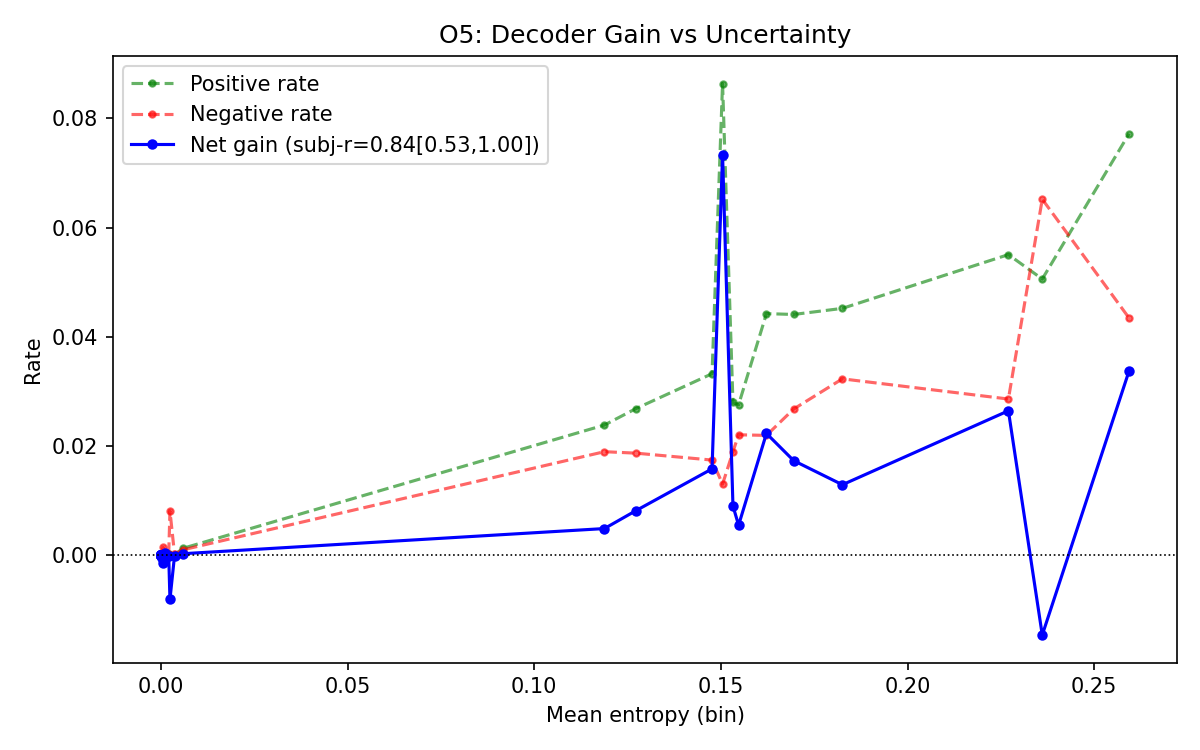
\includegraphics[width=0.42\textwidth]{figures/obs-mednext/O5_decoder_gain.png} &
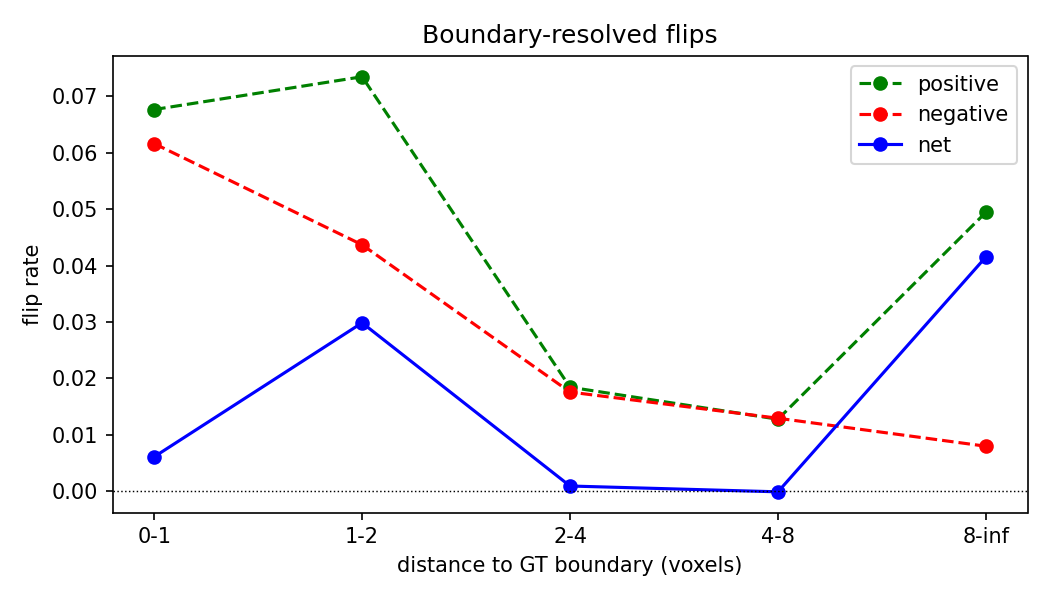
\includegraphics[width=0.42\textwidth]{figures/obs-mednext/O_boundary_flips.png} \\
(e) MedNeXt-M-K3 Global Flips & (f) MedNeXt-M-K3 Boundary Flips \\
\end{tabular}
\caption{Voxel-level net gain (left column) and spatial ground-truth boundary concentration (right column) across 3D UX-Net, SwinUNETR, and MedNeXt-M-K3 backbones under Full ($E_0$) vs. Efficient ($E_1$) decoders.}
\label{fig:heterogeneity}
\end{figure*}

\subsubsection{Anatomical Structure Volatility}
Anatomical analysis (Figure \ref{fig:heterogeneity_anatomy}) demonstrates that small, morphologically complex organs exhibit high flip volatility. The left and right adrenal glands show positive correction rates of 16.2\%/16.9\% in 3D UX-Net, 14.4\%/14.8\% in SwinUNETR, and 18.3\%/10.4\% in MedNeXt-M-K3. Conversely, large structures like the liver remain highly stable ($<3\%$ correctness activity).

\begin{figure*}[tb]
\centering

\includegraphics[width=0.85\textwidth]{figures/obs-uxnet-concat/O_anatomy.png} \\
\vspace{-2pt}{\small (a) 3D UX-Net Organ-Level Flips} \\[4pt]

\includegraphics[width=0.85\textwidth]{figures/obs-swin-concat/O_anatomy.png} \\
\vspace{-2pt}{\small (b) SwinUNETR Organ-Level Flips} \\[4pt]
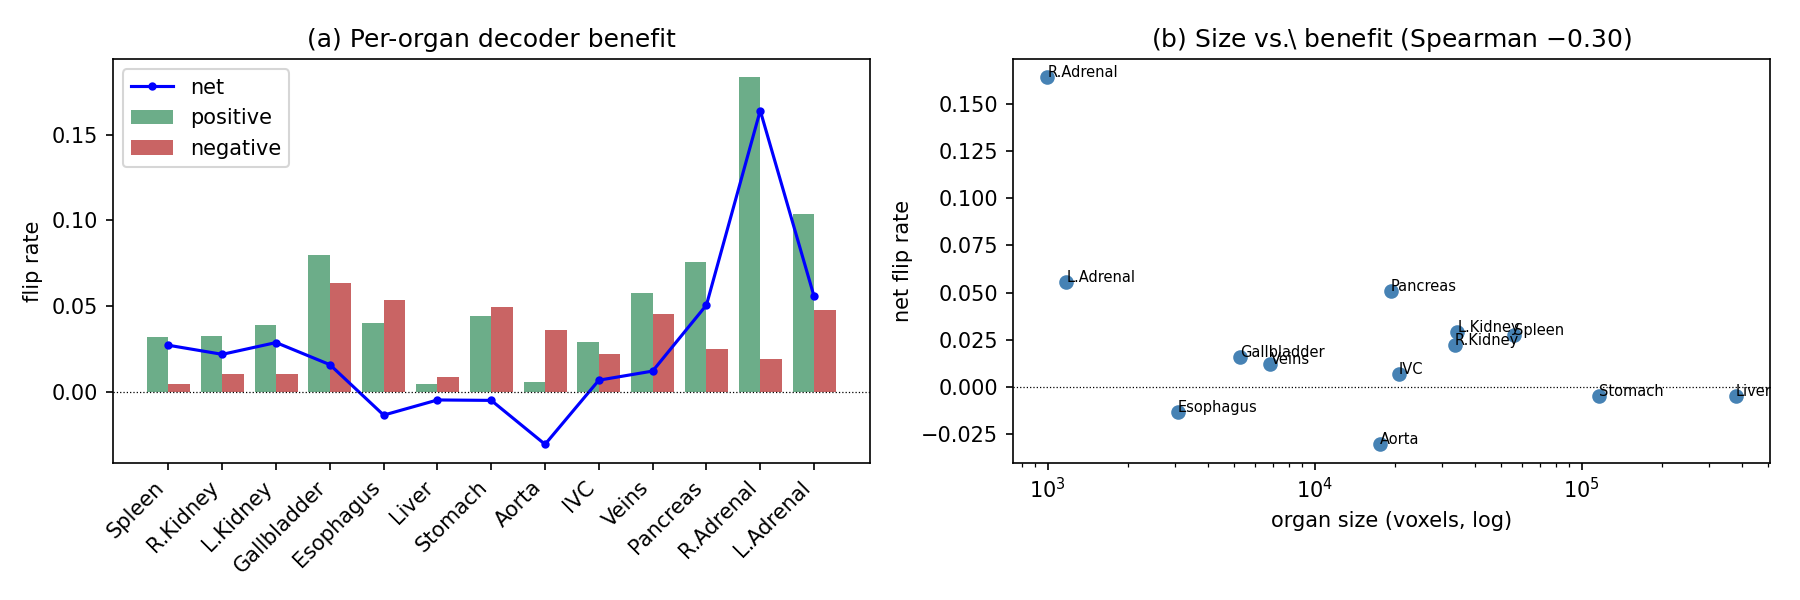
\includegraphics[width=0.85\textwidth]{figures/obs-mednext/O_anatomy.png} \\
\vspace{-2pt}{\small (c) MedNeXt-M-K3 Organ-Level Flips} \\
\caption{Organ-level flip breakdown across backbones on the BTCV CT multi-organ dataset under Full ($E_0$) vs. Efficient ($E_1$) decoders.}
\label{fig:heterogeneity_anatomy}
\end{figure*}

\subsection{Frozen-Encoder Factor Attribution and Interaction Analysis}
\label{sec:results_factorial}

Table \ref{tab:factorial} reports our $2\times2$ factorial configuration grid on 3D UX-Net with frozen shared encoders on BTCV CT. Table \ref{tab:factorial_effects} presents the main effects and interaction analysis across key outcome metrics:
\begin{itemize}
    \item \textbf{High-Resolution Stage Removal ($RF_1 \rightarrow RF_2$)}: Removing the high-resolution stage accounts for 657.8 GMac $\rightarrow$ 319.1 GMac FLOP savings. Retaining this high-resolution stage yields a net positive correction rate of $+0.033\%$ in the 0--2 mm physical GT boundary band and $+0.031\%$ in the 2--4 mm band, decaying to negative net values ($-0.011\%$) in organ interiors ($>8\text{ mm}$).
    \item \textbf{Channel Width Reduction ($C_{384} \rightarrow C_{48}$)}: Reducing decoder channels compresses parameter count by $95\%$ (46.7M $\rightarrow$ 2.2M) while exerting a spatially diffuse and net-neutral effect ($R_{\text{net}}^{\text{all}} = +0.027\%$, 95\% CI: $[-0.027\%, +0.083\%]$).
\end{itemize}

\begin{table*}[tb]
\centering
\caption{$2\times2$ Factorial analysis of decoder channel reduction ($C_{dec}$) and resolution scaling ($RF$) on 3D UX-Net and BTCV CT (Decoder-Isolated Factor Attribution Axis).}
\label{tab:factorial}
\small
\begin{tabular*}{\textwidth}{@{\extracolsep{\fill}}lcccccc}
\toprule
\textbf{Configuration} & $C_{dec}$ & $RF$ & \textbf{Params (M)} & \textbf{FLOPs (GMac)} & \textbf{Latency (ms)} & \textbf{Mean Dice (\%)} \\
\midrule
Full ($C_{384}, RF_1$) & 384 & 1 & 46.72 & 657.76 & 43.3 & 80.44 \\
Chan-Only ($C_{48}, RF_1$) & 48 & 1 & 2.24 & 388.15 & 35.2 & 79.80 \\
Res-Only ($C_{384}, RF_2$) & 384 & 2 & 46.32 & 319.10 & 16.1 & 77.97 \\
Effi ($C_{48}, RF_2$) & 48 & 2 & 1.84 & 49.49 & 8.0 & 78.35 \\
\bottomrule
\end{tabular*}
\end{table*}

\begin{table}[tb]
\centering
\caption{Factor main effects ($\Delta_C, \Delta_{RF}$) and interaction ($\Delta_{C \times RF}$) across metrics on 3D UX-Net (BTCV CT).}
\label{tab:factorial_effects}
\small
\begin{tabular}{@{}l c c c@{}}
\toprule
\textbf{Outcome Metric} & \textbf{Channel $\Delta_C$} & \textbf{Stage $\Delta_{RF}$} & \textbf{Interaction $\Delta_{C \times RF}$} \\
\midrule
Mean Dice (\%) & $-0.13$ & $-1.96$ & $+1.02$ \\
Params (M) & $-44.48$ & $-0.40$ & $+0.00$ \\
FLOPs (GMac) & $-269.61$ & $-338.66$ & $+0.00$ \\
Boundary Net Gain (\%) & $-0.020$ & $+0.033$ & $-0.004$ \\
\bottomrule
\end{tabular}
\end{table}

\subsection{Positive-Gain Concentration ($K_{80}$)}
\label{sec:results_concentration}

Figure \ref{fig:concentration} presents oracle benefit concentration curves. Across our evaluated benchmark backbones and datasets, an oracle selecting the top 5\% of spatial blocks contains 80\% of the total positive net gain ($K_{80} \le 5\%$). At a 10\% volume budget, oracle coverage reaches 99.98\%.

\begin{figure}[tb]
\centering

\includegraphics[width=0.82\columnwidth]{figures/obs-uxnet-concat/O_pareto.png} \\
\vspace{-2pt}{\small (a) 3D UX-Net Concentration Curve} \\[4pt]

\includegraphics[width=0.82\columnwidth]{figures/obs-swin-concat/O_pareto.png} \\
\vspace{-2pt}{\small (b) SwinUNETR Concentration Curve} \\[4pt]

\includegraphics[width=0.82\columnwidth]{figures/obs-mednext/O_pareto.png} \\
\vspace{-2pt}{\small (c) MedNeXt-M-K3 Concentration Curve}
\caption{Oracle benefit concentration curves ($K_{80}$) across 3D UX-Net, SwinUNETR, and MedNeXt-M-K3.}
\label{fig:concentration}
\end{figure}

\subsection{Predictability and Retrospective Hybrid Recovery}
\label{sec:results_predictability}

We evaluate whether cheap inference-time signals can locate regions where decoder computation alters correctness (Location AUROC) and whether they can further discriminate the direction of those changes (Direction AUROC) (Figure \ref{fig:predictability} and Figure \ref{fig:flip_density}):
\begin{itemize}
    \item \textbf{Activity Location AUROC}: Predictive entropy reliably identifies active blocks ($A_{\text{corr}}(r) > 0$), achieving high location AUROCs of 0.900 for 3D UX-Net (AUPRC 0.371), 0.913 for SwinUNETR (AUPRC 0.351), and 0.931 for MedNeXt-M-K3.
    \item \textbf{Directional Utility Discrimination}: Predictive entropy provides strong activity localization but only weak directional discrimination ($G(r) > 0$ vs. $G(r) < 0$), yielding direction AUROCs modestly above chance: 0.591 for 3D UX-Net, 0.560 for SwinUNETR, and 0.545 for MedNeXt-M-K3.
    \item \textbf{TTA Mutual Information (TTA-MI)}: Multi-sample epistemic disagreement $I(v)$ over $K=8$ spatial view transformations yields modest direction AUROCs of 0.539 for 3D UX-Net and 0.570 for SwinUNETR.
    \item \textbf{Conditional Density Overlap}: Figure \ref{fig:flip_density} visualizes conditional entropy density distributions $p(H \mid P(v)=1)$ and $p(H \mid N(v)=1)$, showing near-identical overlap.
\end{itemize}

\begin{figure}[tb]
\centering

\includegraphics[width=0.82\columnwidth]{figures/obs-uxnet-concat/O3_entropy_by_flip.png} \\
\vspace{-2pt}{\small (a) 3D UX-Net Flip Entropy Density} \\[4pt]

\includegraphics[width=0.82\columnwidth]{figures/obs-swin-concat/O3_entropy_by_flip.png} \\
\vspace{-2pt}{\small (b) SwinUNETR Flip Entropy Density}
\caption{Conditional entropy density distributions for positive corrections ($P$) and negative degradations ($N$).}
\label{fig:flip_density}
\end{figure}

\begin{figure}[tb]
\centering

\includegraphics[width=0.82\columnwidth]{figures/obs-uxnet-concat/O3_unc_error.png} \\
\vspace{-2pt}{\small (a) 3D UX-Net Predictability} \\[4pt]

\includegraphics[width=0.82\columnwidth]{figures/obs-swin-concat/O3_unc_error.png} \\
\vspace{-2pt}{\small (b) SwinUNETR Predictability} \\[4pt]

\includegraphics[width=0.82\columnwidth]{figures/obs-mednext/O3_unc_error.png} \\
\vspace{-2pt}{\small (c) MedNeXt-M-K3 Predictability}
\caption{Inference-time block predictability (Location AUROC vs. Direction AUROC) across backbones.}
\label{fig:predictability}
\end{figure}

\subsubsection{Retrospective Hybrid Dice Gap Recovery ($R_{\text{recovery}}$)}
Figure \ref{fig:macro_recovery} presents retrospective hybrid prediction recovery curves $R_{\text{recovery}}(k)$:
\begin{itemize}
    \item At a \textbf{5\% block budget}, entropy-guided output substitution recovers \textbf{60\% of the full decoder's Dice gap} over $E_1$ for 3D UX-Net (vs. 8\% for random selection).
    \item At a \textbf{20\% block budget}, entropy-guided output substitution achieves \textbf{100\% recovery of the macro Dice gap} across our evaluated BTCV backbones (3D UX-Net and SwinUNETR, vs. 17--20\% for random selection).
\end{itemize}

\begin{figure}[tb]
\centering

\includegraphics[width=0.82\columnwidth]{figures/obs-uxnet-concat/R_recovery.png} \\
\vspace{-2pt}{\small (a) 3D UX-Net Macro Dice Recovery} \\[4pt]

\includegraphics[width=0.82\columnwidth]{figures/obs-swin-concat/R_recovery.png} \\
\vspace{-2pt}{\small (b) SwinUNETR Macro Dice Recovery}
\caption{Macro-metric Dice recovery curves ($R_{\text{recovery}}$) under retrospective entropy-guided output hybridization vs. random selection.}
\label{fig:macro_recovery}
\end{figure}
